\section{Navigation}\label{navigation}

To set the current view there are two elements:

\begin{description}
	\item[Camera]\index{navigation!camera} represents a point where the camera is located
	\item[Target]\index{navigation!target} represents the point onto which the camera will focus (the
	camera is \emph{always} looking at the target.)
\end{description}

\subsection{Camera and Target movement
	step}\label{camera-and-target-movement-step}

The relationship between the camera point and the target point can be altered
manually by changing the numbers in the edit fields, or by navigating with
distance and rotation ``steps'' defined by the user.

For rotations, the camera is moved by the parameter \textbf{rotation step}
(default 15 degrees). For movements of the camera and/or the target in a linear
direction, the parameter \textbf{step} (default 0.5) is used. There are two
modes for its use:

\subsubsection{Relative step mode}\label{relative-step-mode}\index{navigation!relative step}

The \textbf{step} for moving the camera and/or target in a linear direction is
calculated relative to the estimated distance from the surface of the fractal.
The closer to the surface that the camera is located, the smaller the step. This
prevents movement of the camera beneath the surface of fractal, because very
close to the surface, a step needs to be very small.

The actual step is equal to the distance from the fractal multiplied by the
parameter \textbf{step}.

Example: If in this mode, the step is set at 0.5 and the nearest point of the
fractal is 3.0, this camera will be moved 1.5 (no matter in which direction).

Relative step mode makes navigation easier, because a user don't need to think
how much camera have to be moved to not hit the fractal surface.

In animations this mode is recommended when camera is approaching the surface of
the fractal.

\subsubsection{Absolute step mode}\label{absolute-step-mode}\index{navigation!absolute step}

Step movement of the camera and/or target is fixed. Therefore if the step is set
at 0.5, the movement will be 0.5 in the direction of the arrow key or mouse
pointer.

This mode is recommended for animation camera flying with a fixed (or strictly
controlled) speed.

\subsection{Linear camera and target movement modes using the arrow
	buttons}\label{linear-camera-and-target-movement-modes-using-the-arrow-buttons}

A user can navigate by operating the arrow keys on the Navigation dock, with the
user defined steps.

There are three modes for changing the relationship between camera and target.
\begin{itemize}
	\item move camera and target
	\item move only camera
	\item move only target
\end{itemize}

\subsubsection{Move camera and target mode}\label{move-camera-and-target-mode}\index{navigation!camera}
\nopagebreak

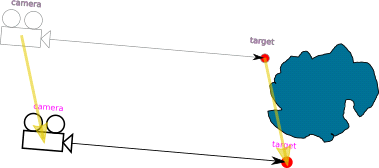
\includegraphics[width=0.5\linewidth]{img/manual/media/move_camera_and_target}
\nopagebreak

Movement mode - \emph{camera and target}
\nopagebreak

Arrows move both the camera and the target by the same distance in the same
direction. The angle of camera rotation does not change.


\subsubsection{Move camera mode}\label{move-camera-mode}\index{navigation!camera}
\nopagebreak

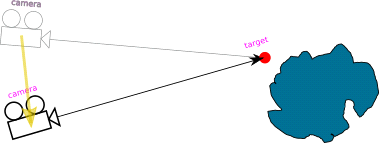
\includegraphics[width=0.5\linewidth]{img/manual/media/move_only_camera}
\nopagebreak

Movement mode - \textit{camera}
\nopagebreak

Moves only the camera and rotates it in respect to the motionless target.

\subsubsection{Move target mode}\label{move-target-mode}\index{navigation!target}
\nopagebreak

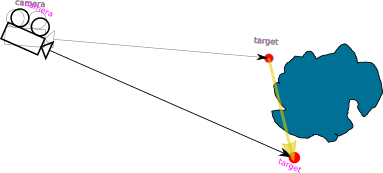
\includegraphics[width=0.5\linewidth]{img/manual/media/move_target}
\nopagebreak

Movement mode - \emph{target}
\nopagebreak

Moves only the target while maintaining a fixed camera position. The camera
rotates following the target. \textbf{Note:} In Relative Step Mode, the target
is moved by distance related to distance of target to fractal surface. If target
is inside the fractal (distance = 0), then this option will not work with
Relative Step Mode.

\subsection{Linear camera and target movement modes using the mouse
	pointer}\label{linear-camera-and-target-movement-modes-using-the-mouse-pointer}

A user can move the camera by indicating point on image and use left mouse
button (go forward) or right button (go backward).


\subsubsection{Move camera and target mode}\label{move-camera-and-target-mode-1}

The target is moved to the point selected by the mouse. The camera is moved
towards selected point by a user defined step, and rotated.

In relative step mode, the camera is moved by distance equals to
\emph{distance\_to\_indicated\_point} multiplied by \emph{step} parameter.

In absolute step mode, the camera is moved by distance equals to \emph{step}
parameter.

\subsubsection{Move camera mode}\label{move-camera-mode-1}

The camera is moved by the step (absolute or relative) in the direction of the
mouse pointer, rotating the camera to look at the target. The target remains
stationary.

\subsubsection{Move target mode}\label{move-target-mode-1}

The target is moved to the point selected by the mouse. The camera remains at
the same point but rotates following the target.

\subsection{Camera rotation modes using the arrow
	buttons}\label{camera-rotation-modes-using-the-arrow-buttons}

\subsubsection{Rotate camera}\label{rotate-camera}\index{navigation!rotate}
\nopagebreak

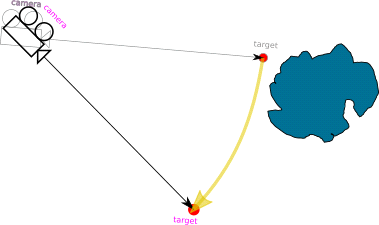
\includegraphics[width=0.5\linewidth]{img/manual/media/rotate_camera}
\nopagebreak

Rotation mode - \emph{around camera}
\nopagebreak

The camera is rotated by the rotation step around its axis and the target is
moved accordingly. This is the standard mode for rotation of the camera.

\subsubsection{Rotate around target}\label{rotate-around-target}
\nopagebreak

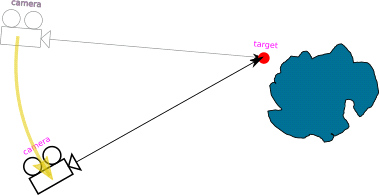
\includegraphics[width=0.5\linewidth]{img/manual/media/rotate_around_target}
\nopagebreak

Rotation mode - \emph{around target}
\nopagebreak

The camera is moved around the stationary target by the rotation step,
maintaining a constant distance to the target. The camera is rotated to look at
the target.

\subsection{Reset View}\label{reset-view}\index{navigation!reset view}

Camera Position is reset, by being zoomed out from the fractal but still
maintaing the camera angles.

If the rotations are changed to zero before using Reset View, the camera will
then be zoomed out from the target, and rotated to look down the y axis.

\subsection{Calculation of rotation angles
	modes}\label{calculation-of-rotation-angles-modes}

\subsubsection{Fixed-roll angle}\label{fixed-roll-angle}

In this mode, the angle gamma (roll) is constant. Pan the camera left or right
always takes place around the global vertical Z-axis (not the render window
vertical axis).

This mode can be likened to an aircrafts controls, where all turns are relative
to the aircraft's axis, not the ground below. Rotate up / down raises / lowers
the nose of the aircraft. Rotate left / right turns in the directions of the
wings. Tilting the camera buttons

\includegraphics[width=0.20000in,height=0.20000in]{img/manual/media/button_roll_left.png}
\includegraphics[width=0.20000in,height=0.20000in]{img/manual/media/button_roll_right.png}
tilts the aircraft

When the camera is pointing straight up or down, or when it is upside down in
this mode, it is quite difficult to predict the result of the turn.

\subsubsection{Straight rotation}\label{straight-rotation}

The camera is rotated around its own local axis (local vertical axis is the
render window vertical axis.)

This mode is a more intuitive way to rotate the camera, e.g., turn the camera
left always give the visual effect of the camera rotating in that direction. The
rotation angles are automatically converted so they are appropriate for the
selected direction. This mode changes the gamma angle (roll).

\subsection{Camera rotation in animations}\label{camera-rotation-in-animations}\index{animation!rotation}

With animation, the camera point and the target point can move independently
following their own trajectories, with the camera always looking towards the
target point. It is important to be aware that the rotation angle of the camera
is the result of the camera coordinates and the target coordinates.

There are various ways of animating, depending on the objective.

The following example is a flight animation, with the camera trajectory
approaching a location, with the camera rotating simultaneously so that the
location is always observed, (as shown in the figure below). The camera
positions represent three keyframes.

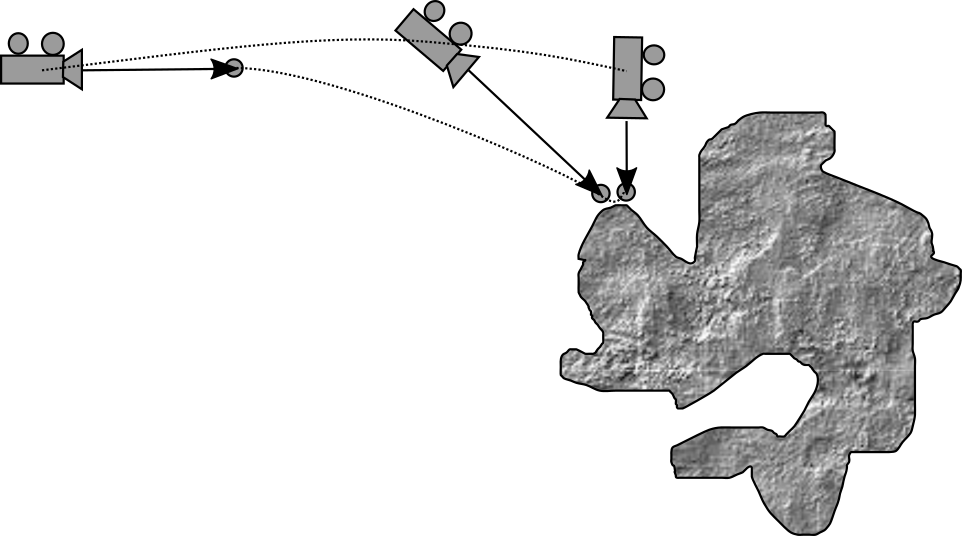
\includegraphics[width=0.7\linewidth]{img/manual/media/camera_target_tracking.png}

Keyframe Animation with differing distances camera to target

Between the first and second keyframes, the camera and target both move large
distances. But between the second and third keyframes, the camera moves a much
greater distance than the target. This can sometimes lead to unexpected camera
rotations between keyframes.

To compensate for this, on the Keyframe navigation tab use the button \emph{Set the
same distance from the camera for all the frames} This adjusts all keyframes by
setting a constant distance between camera and target. It is important to note
that the use of this function does not change the visual effect for the
keyframes, and will help correct interpolation.
\nopagebreak

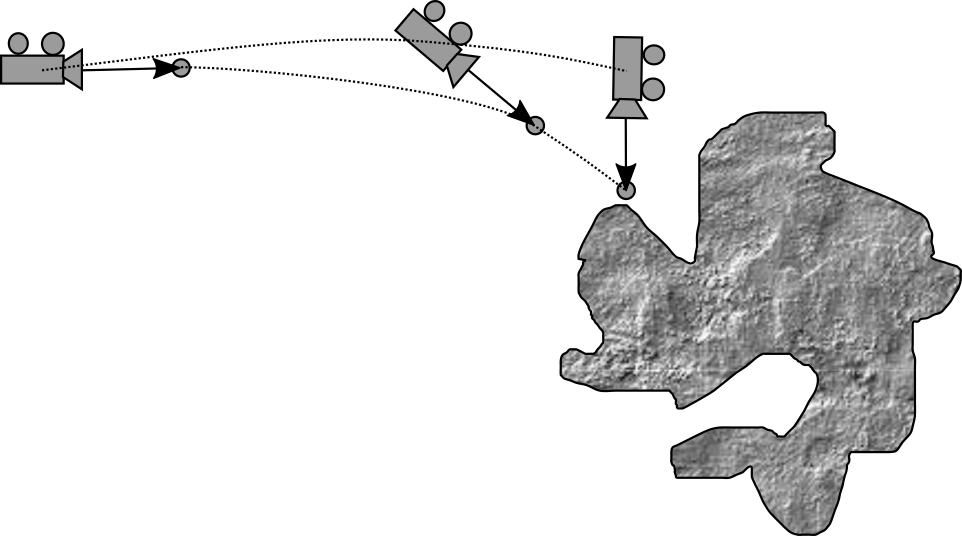
\includegraphics[width=0.7\linewidth]{img/manual/media/camera_target_tracking_2.png}
